% Options for packages loaded elsewhere
\PassOptionsToPackage{unicode}{hyperref}
\PassOptionsToPackage{hyphens}{url}
\PassOptionsToPackage{dvipsnames,svgnames*,x11names*}{xcolor}
%
\documentclass[
  11pt,
]{scrartcl}
\usepackage{lmodern}
\usepackage{setspace}
\usepackage{amsmath}
\usepackage{ifxetex,ifluatex}
\ifnum 0\ifxetex 1\fi\ifluatex 1\fi=0 % if pdftex
  \usepackage[T1]{fontenc}
  \usepackage[utf8]{inputenc}
  \usepackage{textcomp} % provide euro and other symbols
  \usepackage{amssymb}
\else % if luatex or xetex
  \usepackage{unicode-math}
  \defaultfontfeatures{Scale=MatchLowercase}
  \defaultfontfeatures[\rmfamily]{Ligatures=TeX,Scale=1}
\fi
% Use upquote if available, for straight quotes in verbatim environments
\IfFileExists{upquote.sty}{\usepackage{upquote}}{}
\IfFileExists{microtype.sty}{% use microtype if available
  \usepackage[]{microtype}
  \UseMicrotypeSet[protrusion]{basicmath} % disable protrusion for tt fonts
}{}
\usepackage{xcolor}
\IfFileExists{xurl.sty}{\usepackage{xurl}}{} % add URL line breaks if available
\IfFileExists{bookmark.sty}{\usepackage{bookmark}}{\usepackage{hyperref}}
\hypersetup{
  pdftitle={Writing a reproducible research paper},
  pdfkeywords={Bookdown, Reproducible research, Template, Manuscript},
  colorlinks=true,
  linkcolor=Maroon,
  filecolor=Maroon,
  citecolor=Blue,
  urlcolor=Blue,
  pdfcreator={LaTeX via pandoc}}
\urlstyle{same} % disable monospaced font for URLs
\usepackage[left=2.5cm, right=2.5cm, top=2.5cm, bottom=4cm]{geometry}
\usepackage{color}
\usepackage{fancyvrb}
\newcommand{\VerbBar}{|}
\newcommand{\VERB}{\Verb[commandchars=\\\{\}]}
\DefineVerbatimEnvironment{Highlighting}{Verbatim}{commandchars=\\\{\}}
% Add ',fontsize=\small' for more characters per line
\usepackage{framed}
\definecolor{shadecolor}{RGB}{248,248,248}
\newenvironment{Shaded}{\begin{snugshade}}{\end{snugshade}}
\newcommand{\AlertTok}[1]{\textcolor[rgb]{0.94,0.16,0.16}{#1}}
\newcommand{\AnnotationTok}[1]{\textcolor[rgb]{0.56,0.35,0.01}{\textbf{\textit{#1}}}}
\newcommand{\AttributeTok}[1]{\textcolor[rgb]{0.77,0.63,0.00}{#1}}
\newcommand{\BaseNTok}[1]{\textcolor[rgb]{0.00,0.00,0.81}{#1}}
\newcommand{\BuiltInTok}[1]{#1}
\newcommand{\CharTok}[1]{\textcolor[rgb]{0.31,0.60,0.02}{#1}}
\newcommand{\CommentTok}[1]{\textcolor[rgb]{0.56,0.35,0.01}{\textit{#1}}}
\newcommand{\CommentVarTok}[1]{\textcolor[rgb]{0.56,0.35,0.01}{\textbf{\textit{#1}}}}
\newcommand{\ConstantTok}[1]{\textcolor[rgb]{0.00,0.00,0.00}{#1}}
\newcommand{\ControlFlowTok}[1]{\textcolor[rgb]{0.13,0.29,0.53}{\textbf{#1}}}
\newcommand{\DataTypeTok}[1]{\textcolor[rgb]{0.13,0.29,0.53}{#1}}
\newcommand{\DecValTok}[1]{\textcolor[rgb]{0.00,0.00,0.81}{#1}}
\newcommand{\DocumentationTok}[1]{\textcolor[rgb]{0.56,0.35,0.01}{\textbf{\textit{#1}}}}
\newcommand{\ErrorTok}[1]{\textcolor[rgb]{0.64,0.00,0.00}{\textbf{#1}}}
\newcommand{\ExtensionTok}[1]{#1}
\newcommand{\FloatTok}[1]{\textcolor[rgb]{0.00,0.00,0.81}{#1}}
\newcommand{\FunctionTok}[1]{\textcolor[rgb]{0.00,0.00,0.00}{#1}}
\newcommand{\ImportTok}[1]{#1}
\newcommand{\InformationTok}[1]{\textcolor[rgb]{0.56,0.35,0.01}{\textbf{\textit{#1}}}}
\newcommand{\KeywordTok}[1]{\textcolor[rgb]{0.13,0.29,0.53}{\textbf{#1}}}
\newcommand{\NormalTok}[1]{#1}
\newcommand{\OperatorTok}[1]{\textcolor[rgb]{0.81,0.36,0.00}{\textbf{#1}}}
\newcommand{\OtherTok}[1]{\textcolor[rgb]{0.56,0.35,0.01}{#1}}
\newcommand{\PreprocessorTok}[1]{\textcolor[rgb]{0.56,0.35,0.01}{\textit{#1}}}
\newcommand{\RegionMarkerTok}[1]{#1}
\newcommand{\SpecialCharTok}[1]{\textcolor[rgb]{0.00,0.00,0.00}{#1}}
\newcommand{\SpecialStringTok}[1]{\textcolor[rgb]{0.31,0.60,0.02}{#1}}
\newcommand{\StringTok}[1]{\textcolor[rgb]{0.31,0.60,0.02}{#1}}
\newcommand{\VariableTok}[1]{\textcolor[rgb]{0.00,0.00,0.00}{#1}}
\newcommand{\VerbatimStringTok}[1]{\textcolor[rgb]{0.31,0.60,0.02}{#1}}
\newcommand{\WarningTok}[1]{\textcolor[rgb]{0.56,0.35,0.01}{\textbf{\textit{#1}}}}
\usepackage{longtable,booktabs}
% Correct order of tables after \paragraph or \subparagraph
\usepackage{etoolbox}
\makeatletter
\patchcmd\longtable{\par}{\if@noskipsec\mbox{}\fi\par}{}{}
\makeatother
% Allow footnotes in longtable head/foot
\IfFileExists{footnotehyper.sty}{\usepackage{footnotehyper}}{\usepackage{footnote}}
\makesavenoteenv{longtable}
\usepackage{graphicx}
\makeatletter
\def\maxwidth{\ifdim\Gin@nat@width>\linewidth\linewidth\else\Gin@nat@width\fi}
\def\maxheight{\ifdim\Gin@nat@height>\textheight\textheight\else\Gin@nat@height\fi}
\makeatother
% Scale images if necessary, so that they will not overflow the page
% margins by default, and it is still possible to overwrite the defaults
% using explicit options in \includegraphics[width, height, ...]{}
\setkeys{Gin}{width=\maxwidth,height=\maxheight,keepaspectratio}
% Set default figure placement to htbp
\makeatletter
\def\fps@figure{htbp}
\makeatother
\setlength{\emergencystretch}{3em} % prevent overfull lines
\providecommand{\tightlist}{%
  \setlength{\itemsep}{0pt}\setlength{\parskip}{0pt}}
\setcounter{secnumdepth}{-\maxdimen} % remove section numbering

%redefine abstract environment
\renewenvironment{abstract}
 {\vfill
  \begin{center}
  \bfseries \abstractname\vspace{-.5em}\vspace{0pt}
  \end{center}
  \list{}{
    \setlength{\leftmargin}{2cm}%
    \setlength{\rightmargin}{\leftmargin}%
  }%
  \item\relax}
 {\endlist}

%redefine the thanks command
\makeatletter
\def\thanks#1{\protected@xdef\@thanks{\@thanks
        \protect\footnotetext{#1}}}
\makeatother


\usepackage{booktabs}
\usepackage{longtable}
\usepackage{array}
\usepackage{multirow}
\usepackage{wrapfig}
\usepackage{float}
\usepackage{colortbl}
\usepackage{pdflscape}
\usepackage{tabu}
\usepackage{threeparttable}
\usepackage{threeparttablex}
\usepackage[normalem]{ulem}
\usepackage{makecell}
\usepackage{xcolor}
\ifluatex
  \usepackage{selnolig}  % disable illegal ligatures
\fi
\newlength{\cslhangindent}
\setlength{\cslhangindent}{1.5em}
\newlength{\csllabelwidth}
\setlength{\csllabelwidth}{3em}
\newenvironment{CSLReferences}[3] % #1 hanging-ident, #2 entry spacing
 {% don't indent paragraphs
  \setlength{\parindent}{0pt}
  % turn on hanging indent if param 1 is 1
  \ifodd #1 \everypar{\setlength{\hangindent}{\cslhangindent}}\ignorespaces\fi
  % set entry spacing
  \ifnum #2 > 0
  \setlength{\parskip}{#2\baselineskip}
  \fi
 }%
 {}
\usepackage{calc} % for \widthof, \maxof
\newcommand{\CSLBlock}[1]{#1\hfill\break}
\newcommand{\CSLLeftMargin}[1]{\parbox[t]{\maxof{\widthof{#1}}{\csllabelwidth}}{#1}}
\newcommand{\CSLRightInline}[1]{\parbox[t]{\linewidth}{#1}}
\newcommand{\CSLIndent}[1]{\hspace{\cslhangindent}#1}

\title{Writing a reproducible research paper\thanks{The acknowledgments go to everyone involved in creating free and open software and, in particular, to the author of the great bookdown page Yihui Xie.}}
\author{Julia Schulte-Cloos}
\date{2020-11-13}

\begin{document}
\maketitle
\begin{abstract}
Everyone agrees that this issue is really important. But we do not know much about this specific question, although it matters a great deal, for these reasons. We approach the problem from this perspective. Our research design focuses on these cases and relies on these data, which we analyse using this method. Results show what we have learned about the question. They have these broader implications.

\textbf{Keywords}: Bookdown, Reproducible research, Template, Manuscript

Dr.~Julia Schulte-Cloos
Marie Curie Research Fellow, Geschwister Scholl Institute of Political Science, Ludwig Maxmilian University of Munich, Germany.
E-Mail: \href{mailto:julia.schulte-cloos@gsi.lmu.de}{\nolinkurl{julia.schulte-cloos@gsi.lmu.de}}
ORCID: 0000-0001-7223-3602
\end{abstract}


\thispagestyle{empty}
\setcounter{page}{0}


\setstretch{1.2}
\newpage

\hypertarget{the-basics}{%
\section{The basics}\label{the-basics}}

This is a \LaTeX based manuscript that is generated from an Rmd-file by relying on Pandoc for conversion from Markdown to Tex. If you do not specify a \texttt{template.tex} in your \texttt{YAML} header, Pandoc will use the \texttt{default.latex} template, which you can find \href{https://github.com/jgm/pandoc-templates/blob/master/default.latex}{here}. I suggest that you start writing reproducible research papers with a solid template that achieves most of your needs for producing a good-looking manuscript, but that you focus on integrating code and content over optimizing the beauty of your document. At the end of the document, you find a code chunk in which you can customize and modify the \LaTeX code that will be written to the \texttt{preamble.tex} file that we import in to our reproducible manuscript in the YAML header. I recommend that you make any changes to this preamble there to maintain a single Rmd file that you can re-use for different projects without having to drag too many single files along with the Rmd file in the different directories.

\hypertarget{citations}{%
\subsection{Citations}\label{citations}}

Markdown provides an easy way to cite and reference literature. We add a \texttt{bib}-file in our YAML header in the following way:

\begin{Shaded}
\begin{Highlighting}[]
\SpecialCharTok{{-}{-}{-}}
\NormalTok{output}\SpecialCharTok{:}
\NormalTok{  bookdown}\SpecialCharTok{::}\NormalTok{pdf\_document2}\SpecialCharTok{:}
\NormalTok{csl}\SpecialCharTok{:} \StringTok{\textquotesingle{}assets/sage{-}harvard.csl\textquotesingle{}} 
\NormalTok{bibliography}\SpecialCharTok{:}\NormalTok{ literature.bib  }
\NormalTok{link}\SpecialCharTok{{-}}\NormalTok{citations}\SpecialCharTok{:}\NormalTok{ yes }
\SpecialCharTok{{-}{-}{-}}
\end{Highlighting}
\end{Shaded}

We can then cite all entries included in our \texttt{.bib}-file by calling \texttt{@palmerdata.2020} for inline citations and \texttt{{[}@palmerdata.2020,\ p.10{]}} for all other references. Here is an example: the dataset that we use has been created by \protect\hyperlink{ref-palmerdata.2020}{Horst et al.} (\protect\hyperlink{ref-palmerdata.2020}{2020}). If our document specifies a \href{https://citationstyles.org/}{csl} \href{https://www.zotero.org/styles}{style}, Pandoc will convert Markdown references, i.e., \texttt{@palmerdata.2020}, to `hardcoded' text and a hyperlink to the reference section in our document. If our document, in contrast, specifies a citation reference package like \texttt{biblatex} or \texttt{natbib} along with the related options, pandoc will create the corresponding LaTeX commands (e.g.~\texttt{\textbackslash{}autocite}, or \texttt{\textbackslash{}pcite}) to create the references from our Markdown references.

\hypertarget{figures-and-images}{%
\subsection{Figures and images}\label{figures-and-images}}

There are several different ways to include images in Rmd documents. For PDF outputs, like \texttt{bookdown::pdf\_document2}, we can rely on

\begin{enumerate}
\def\labelenumi{\arabic{enumi}.}
\tightlist
\item
  Plain markdown syntax: \texttt{!{[}A\ cow\textquotesingle{}s\ nose{]}(figs/cow.jpg)\{width=30\%\}}
\end{enumerate}

\begin{figure}
\centering
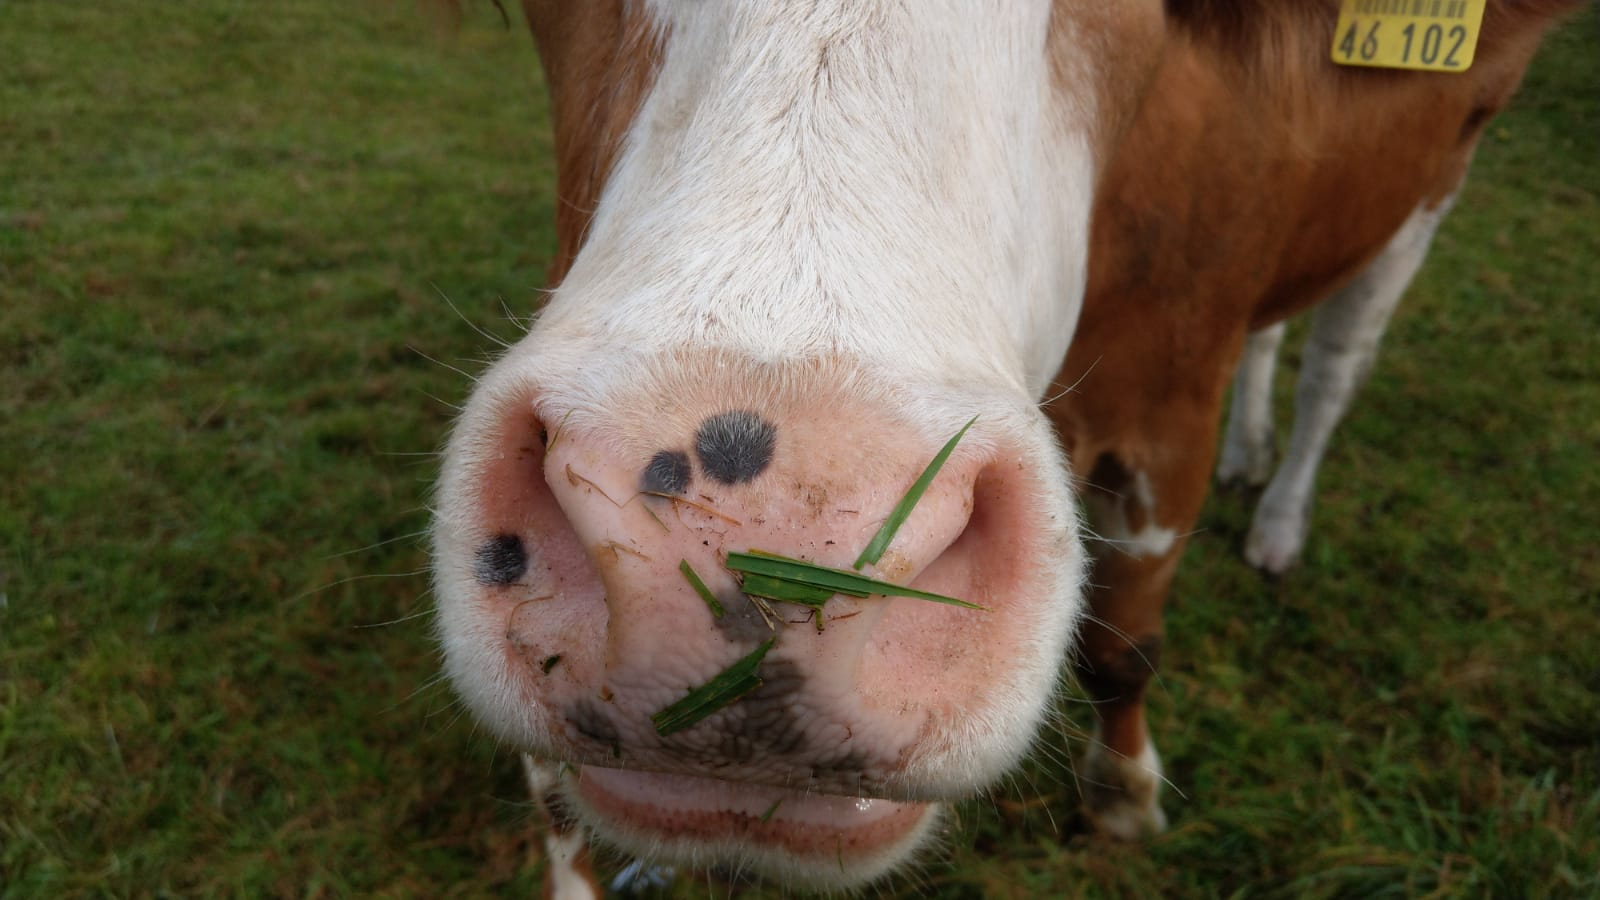
\includegraphics[width=0.3\textwidth,height=\textheight]{figs/cow.jpg}
\caption{A cow's nose}
\end{figure}

\begin{enumerate}
\def\labelenumi{\arabic{enumi}.}
\setcounter{enumi}{1}
\tightlist
\item
  \LaTeX syntax
\end{enumerate}

\begin{Shaded}
\begin{Highlighting}[]
\NormalTok{\textbackslash{}begin\{figure\}}
\NormalTok{\textbackslash{}centering}
\NormalTok{\textbackslash{}includegraphics[width}\OtherTok{=}\FloatTok{0.3}\NormalTok{\textbackslash{}textwidth]\{.}\SpecialCharTok{/}\NormalTok{figs}\SpecialCharTok{/}\NormalTok{snake.jpg\}}
\NormalTok{\textbackslash{}caption\{A snake\}}
\NormalTok{\textbackslash{}end\{figure\}}
\end{Highlighting}
\end{Shaded}

\begin{figure}
\centering
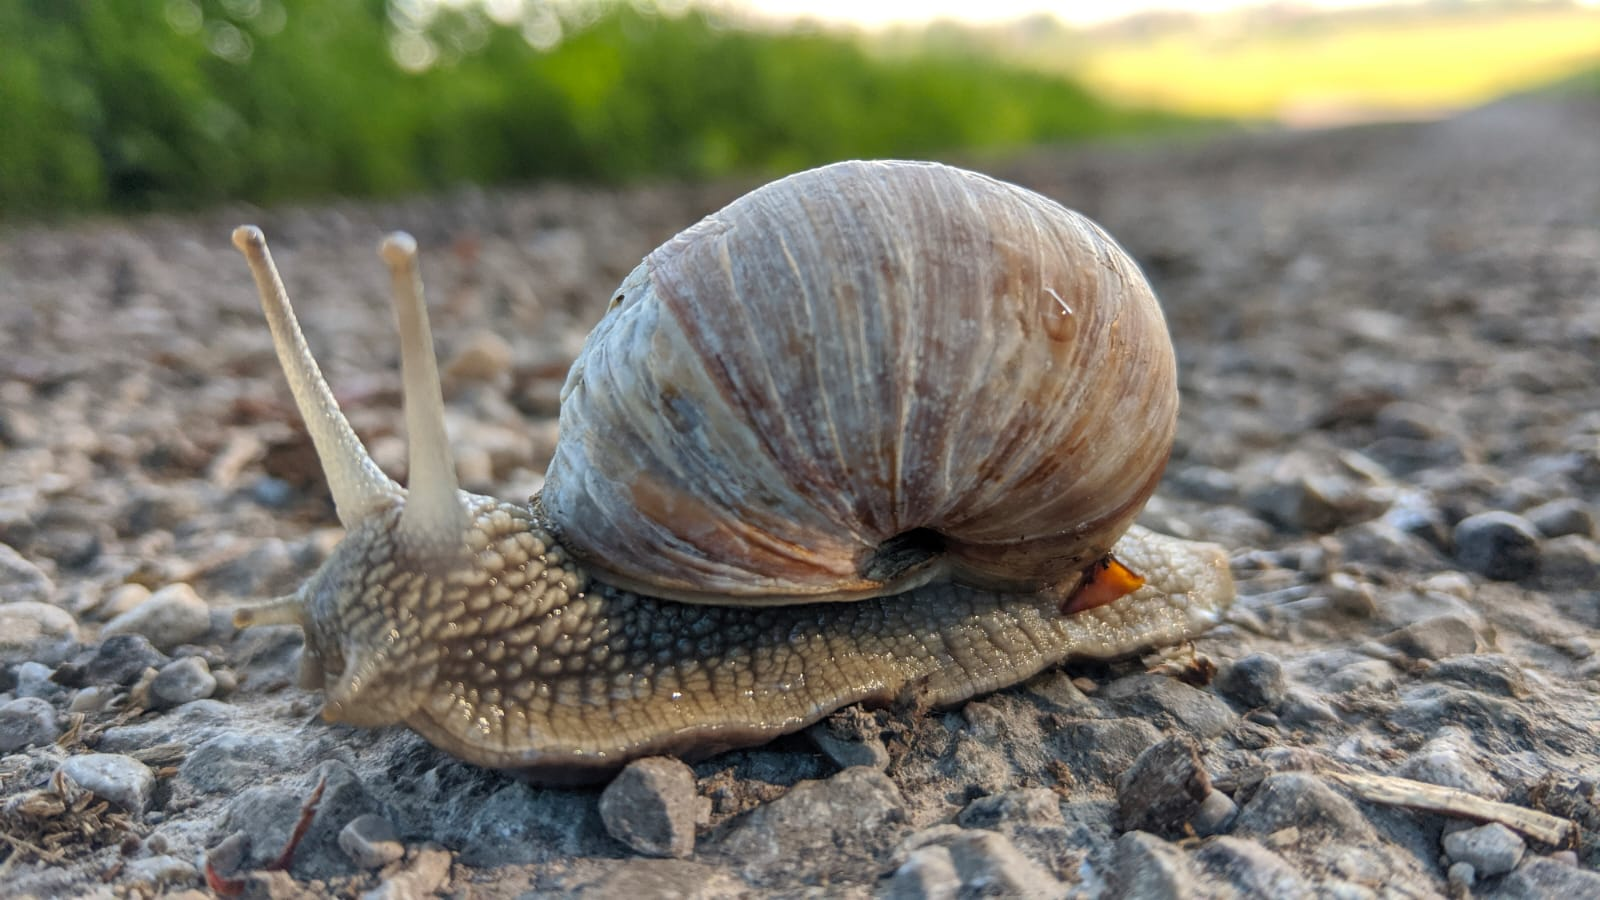
\includegraphics[width=0.3\textwidth]{./figs/snake.jpg}
\caption{A snake}
\end{figure}

\begin{enumerate}
\def\labelenumi{\arabic{enumi}.}
\setcounter{enumi}{2}
\tightlist
\item
  Code evaluation and \texttt{knitr}
\end{enumerate}

\begin{Shaded}
\begin{Highlighting}[]
\NormalTok{knitr}\SpecialCharTok{::}\FunctionTok{include\_graphics}\NormalTok{(}\AttributeTok{path =} \StringTok{"figs/winter.jpg"}\NormalTok{)}
\end{Highlighting}
\end{Shaded}

\begin{figure}

{\centering 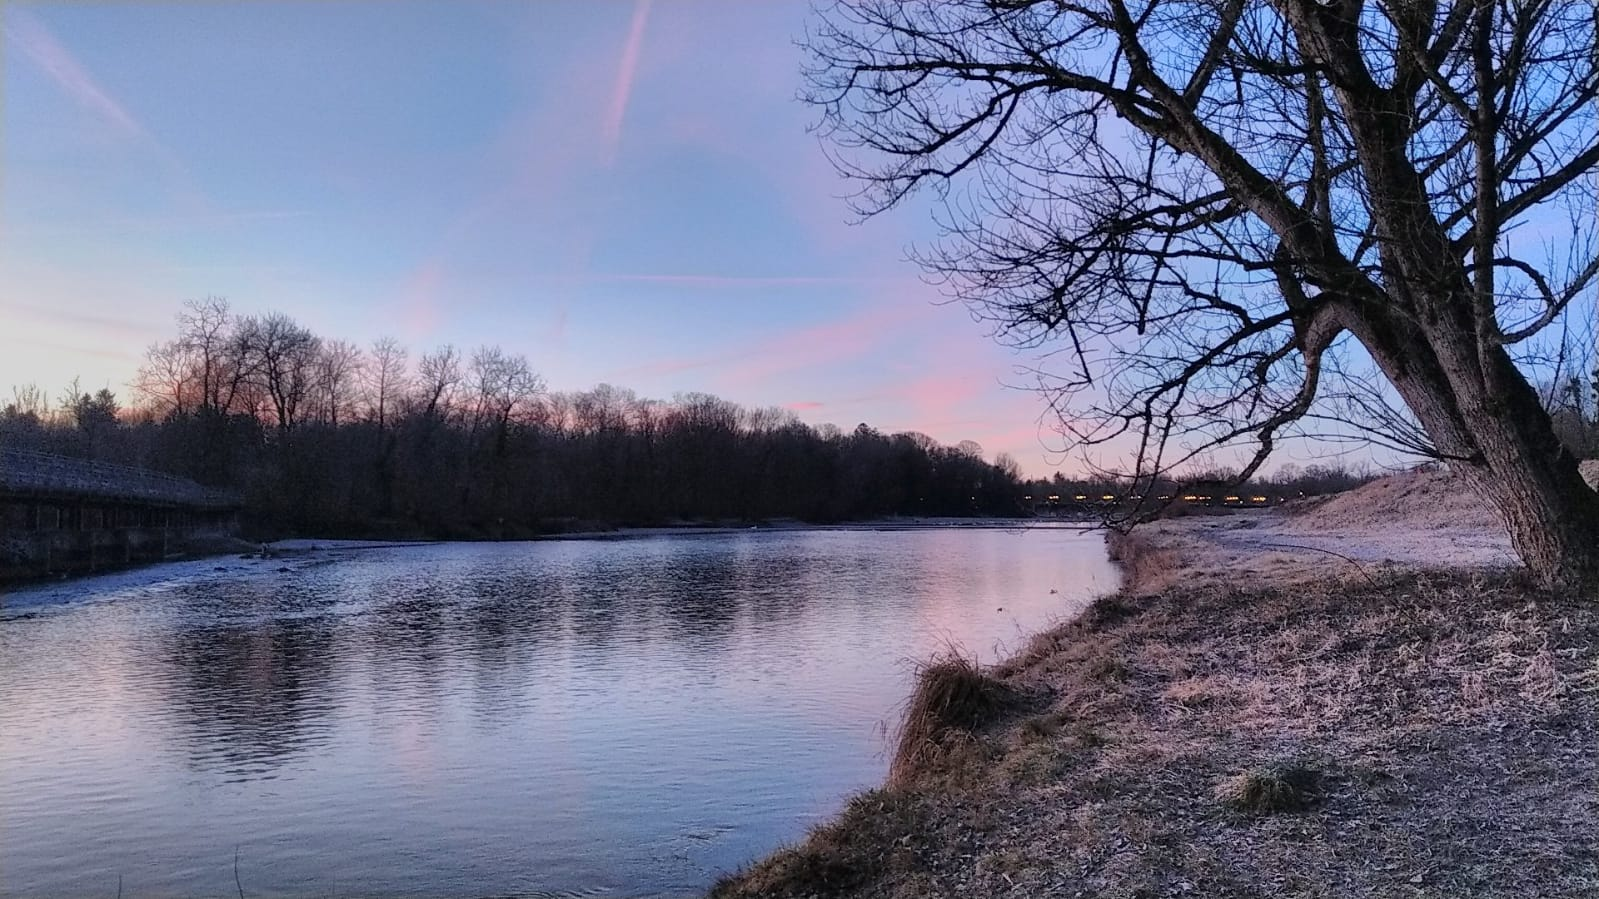
\includegraphics[width=0.3\linewidth]{figs/winter} 

}

\caption{A winter morning}\label{fig:winter}
\end{figure}

\hypertarget{cross-referencing}{%
\subsubsection{Cross-referencing}\label{cross-referencing}}

Cross-referencing is possible in PDF documents when we rely on \texttt{bookdown::pdf\_document2}. We can cross-reference sections, figures, tables or equations in our document with the following syntax: \texttt{\textbackslash{}@ref(fig:winter)}. Here is an example: Figure \ref{fig:winter} shows a photograph of Munich on a winter morning. If we specify the \texttt{colorlinks:\ true} option in our YAML header, the hyperlinks to the respective figure will be colored.

Similarly, we can also cross-reference sections, tables or equations. If you do not specify a section label, Pandoc will automatically assign a label based on the title of your header. For more details, see the \href{https://pandoc.org/MANUAL.html\#extension-auto_identifiers}{Pandoc manual}. If you wish to add a manual label to a header, add \texttt{\{\#mylabel\}} to the end of the section header. If you wish to make reference to an equation, you can rely on \LaTeX syntax and put your equations in equation environments and assign a label by \texttt{(\textbackslash{}\#eq:label)}, e.g.,

\begin{Shaded}
\begin{Highlighting}[]
\NormalTok{\textbackslash{}begin\{equation\} }
\NormalTok{  f\textbackslash{}}\FunctionTok{left}\NormalTok{(k\textbackslash{}right) }\OtherTok{=}\NormalTok{ \textbackslash{}binom\{n\}\{k\} p}\SpecialCharTok{\^{}}\NormalTok{k\textbackslash{}}\FunctionTok{left}\NormalTok{(}\DecValTok{1}\SpecialCharTok{{-}}\NormalTok{p\textbackslash{}right)}\SpecialCharTok{\^{}}\NormalTok{\{n}\SpecialCharTok{{-}}\NormalTok{k\}}
\NormalTok{  (\textbackslash{}}\CommentTok{\#eq:binom)}
\NormalTok{\textbackslash{}end\{equation\} }
\end{Highlighting}
\end{Shaded}

\hypertarget{integrating-code-and-content}{%
\section{Integrating code and content}\label{integrating-code-and-content}}

\emph{Literate programming} is key to reproducible documents, which means that we can integrate our code and text into a single document. We can then also include any kind of operations directly in the text by calling R with a single backtick:

\begin{Shaded}
\begin{Highlighting}[]
\StringTok{\textasciigrave{}}\AttributeTok{r (2+2)*5}\StringTok{\textasciigrave{}}
\end{Highlighting}
\end{Shaded}

Here is an applied example. Let's calculate the mean bill length of penguins in the data and share this information with the readers, while rounding the number to two digits: 43.9219 mm.

\newpage

\hypertarget{graphs---ggplot}{%
\section{\texorpdfstring{Graphs - \texttt{ggplot}}{Graphs - ggplot}}\label{graphs---ggplot}}

\begin{figure}

{\centering \includegraphics[width=0.9\linewidth]{figs/figggplot-1} 

}

\caption{Body mass and flipper length of penguins.}\label{fig:ggplot}
\end{figure}

\hypertarget{tables}{%
\section{Tables}\label{tables}}

In \LaTeX documents, Pandoc will automatically load the packages \texttt{longtable}, \texttt{booktabs}, and \texttt{calc} when we specify the option \texttt{tables:\ yes} in our YAML header.

\hypertarget{including-tables-kable}{%
\subsection{\texorpdfstring{Including tables: \texttt{kable}}{Including tables: kable}}\label{including-tables-kable}}

You can easily create and integrate your tables with the powerful table generating package \texttt{kable} and the table styling package \texttt{kableExtra}. For the full documentation of the package, see the \href{https://haozhu233.github.io/kableExtra/awesome_table_in_pdf.pdf}{vignette}. Here is an example table including some summary statistics of the penguin species.

\begin{table}[!h]

\caption{\label{tab:kable-advanced}Differences in Flipper and Bill Length across Penguin Species}
\centering
\resizebox{\linewidth}{!}{
\begin{tabular}[t]{lrrrr}
\toprule
Species & Bill Length
(mm) & Bill Depth
(mm) & Flipper Length
(mm) & Body Mass
(kg)\\
\midrule
\cellcolor{gray!6}{Adelie} & \cellcolor{gray!6}{38.79} & \cellcolor{gray!6}{18.35} & \cellcolor{gray!6}{189.95} & \cellcolor{gray!6}{3700.66}\\
Chinstrap & 48.83 & 18.42 & 195.82 & 3733.09\\
\cellcolor{gray!6}{Gentoo} & \cellcolor{gray!6}{47.50} & \cellcolor{gray!6}{14.98} & \cellcolor{gray!6}{217.19} & \cellcolor{gray!6}{5076.02}\\
\bottomrule
\end{tabular}}
\end{table}

\hypertarget{including-output-from-regression-tables-modelsummary}{%
\subsection{\texorpdfstring{Including output from regression tables: \texttt{modelsummary}}{Including output from regression tables: modelsummary}}\label{including-output-from-regression-tables-modelsummary}}

\texttt{modelsummary} is a very powerful package to present regression tables in several different output formats. Depending on your preferred table styling package, you can chose among different output formats and then further style the regression table according to your personal needs. In the example below, we use \texttt{kableExtra} to style the table.

\begin{table}[H]
\centering
\begin{tabular}[t]{lcccc}
\toprule
\multicolumn{1}{c}{ } & \multicolumn{2}{c}{Resting Pulse} & \multicolumn{2}{c}{Active Pulse} \\
\cmidrule(l{3pt}r{3pt}){2-3} \cmidrule(l{3pt}r{3pt}){4-5}
  & M1 & M2 & M3 & M4\\
\midrule
(Intercept) & 86.458*** & 86.845*** & 90.769*** & 90.826***\\
 & (4.507) & (4.541) & (9.397) & (9.479)\\
Smoke & 2.048 & -1.515 & 2.406 & 1.883\\
 & (1.816) & (5.060) & (3.786) & (10.563)\\
\textbf{Exercise} & \textbf{-6.853***} & \textbf{-7.046***} & \textbf{-8.657***} & \textbf{-8.685***}\\
 & (0.778) & (0.820) & (1.622) & (1.712)\\
Wgt & -0.022 & -0.021 & 0.097* & 0.097*\\
 & (0.024) & (0.024) & (0.050) & (0.051)\\
Sex & 1.175 & 1.189 & 9.430*** & 9.432***\\
 & (1.512) & (1.513) & (3.152) & (3.159)\\
\textbf{Smoke × Exercise} & \textbf{} & \textbf{1.915} & \textbf{} & \textbf{0.281}\\
 &  & (2.539) &  & (5.299)\\
\midrule
R2 & 0.309 & 0.310 & 0.160 & 0.160\\
Num.Obs. & 232 & 232 & 232 & 232\\
\bottomrule
\multicolumn{5}{l}{\textsuperscript{} * p < 0.1, ** p < 0.05, *** p < 0.01}\\
\multicolumn{5}{l}{\textsuperscript{} Dataset: 'Pulse Rates and Exercise' from the Stat2Data package.}\\
\end{tabular}
\end{table}

\newpage

\hypertarget{advanced-literate-programming}{%
\section{Advanced literate programming}\label{advanced-literate-programming}}

\hypertarget{literate-programming-in-figure-captions}{%
\subsection{Literate programming in figure captions}\label{literate-programming-in-figure-captions}}

Sometimes, we would like to include the result of a specific evaluated code in the caption of a figure or a table. We can achieve this, by making use of the code chunk option \texttt{eval.after}. We might, for instance, include the overall number of penguins that are included in the dataset to our earlier Figure \ref{fig:ggplot}.

\begin{figure}

{\centering \includegraphics[width=0.9\linewidth]{figs/figlit-prog-caption-1} 

}

\caption{Body mass and flipper length of penguins. N = 344.}\label{fig:lit-prog-caption}
\end{figure}

\hypertarget{working-with-other-engines-in-rmd}{%
\subsection{Working with other engines in Rmd}\label{working-with-other-engines-in-rmd}}

\hypertarget{python-with-reticulate-package}{%
\subsubsection{\texorpdfstring{Python with \texttt{reticulate} package}{Python with reticulate package}}\label{python-with-reticulate-package}}

The \texttt{reticulate} package allows two-way communication between \texttt{python} and \texttt{R}, thus, you can access any objects created or stored within a \texttt{python}-engine chunk from within an \texttt{R}-enginge chunk, and \emph{vice versa}. To use the \texttt{python}-engine, simply replace the name of the engine after the three backticks and the curyl brace that opens a chunk.

\hypertarget{stata-with-statamarkdown-package}{%
\subsubsection{\texorpdfstring{STATA with \texttt{Statamarkdown} package}{STATA with Statamarkdown package}}\label{stata-with-statamarkdown-package}}

You can also use stata as an engine within your workflow. For more details, you can \href{https://bookdown.org/yihui/rmarkdown-cookbook/eng-stata.html}{consult} the RMarkdown cookbook (\protect\hyperlink{ref-Xie.2020}{Xie et al., 2020: 15.8}).

\begin{Shaded}
\begin{Highlighting}[]
\KeywordTok{sysuse}\NormalTok{ auto}
\KeywordTok{summarize}
\end{Highlighting}
\end{Shaded}

\hypertarget{tweaks-in-rstudio}{%
\section{Tweaks in RStudio}\label{tweaks-in-rstudio}}

There are a number of useful addins in RStudio that facilitate our workflow. You should check out the \texttt{remedy} package if you would like to highlight your code, or insert chunks by point-and-click. The \texttt{styler} package is a useful addin to tidy your code, which is good practice before sharing your scripts.

\newpage

\hypertarget{references}{%
\section{References}\label{references}}

\setlength{\parskip}{10pt}
\setlength{\parindent}{0pt}
\singlespacing

\hypertarget{refs}{}
\begin{CSLReferences}{1}{0}
\leavevmode\hypertarget{ref-palmerdata.2020}{}%
Horst AM, Hill AP and Gorman KB (2020) \emph{Palmerpenguins: Palmer Archipelago (antarctica) Penguin Data}. Available at: \url{https://allisonhorst.github.io/palmerpenguins/}.

\leavevmode\hypertarget{ref-Xie.2020}{}%
Xie Y, Dervieux C and Riederer E (2020) \emph{R Markdown Cookbook}. CRC Press.

\end{CSLReferences}

\newpage

\hypertarget{online-appendix}{%
\section{Online appendix}\label{online-appendix}}

\hypertarget{sec:rsessioninfo}{%
\subsection{Attach R session info in appendix}\label{sec:rsessioninfo}}

Since R and R packages are constantly evolving you might want to add the R session info that contains information on the R version as well as the packages that are loaded.

\begin{verbatim}
R version 4.0.3 (2020-10-10)
Platform: x86_64-w64-mingw32/x64 (64-bit)
Running under: Windows 10 x64 (build 18363)

Locale:
  LC_COLLATE=Portuguese_Portugal.1252  LC_CTYPE=Portuguese_Portugal.1252   
  LC_MONETARY=Portuguese_Portugal.1252 LC_NUMERIC=C                        
  LC_TIME=Portuguese_Portugal.1252    

Package version:
  askpass_1.1          assertthat_0.2.1     backports_1.1.7     
  base64enc_0.1.3      BH_1.72.0.3          blob_1.2.1          
  bookdown_0.21        brew_1.0.6           broom_0.7.0         
  callr_3.4.4          cellranger_1.1.0     checkmate_2.0.0     
  cli_2.0.2            clipr_0.7.0          colorspace_1.4-1    
  commonmark_1.7       compiler_4.0.3       covr_3.5.1          
  crayon_1.3.4         crosstalk_1.1.0.1    curl_4.3            
  DBI_1.1.0            dbplyr_1.4.4         desc_1.2.0          
  devtools_2.3.2       digest_0.6.25        dplyr_1.0.2         
  DT_0.15              ellipsis_0.3.1       evaluate_0.14       
  fansi_0.4.1          farver_2.0.3         forcats_0.5.0       
  fs_1.5.0             generics_0.0.2       ggplot2_3.3.2       
  gh_1.1.0             git2r_0.27.1         glue_1.4.2          
  graphics_4.0.3       grDevices_4.0.3      grid_4.0.3          
  gridExtra_2.3        gtable_0.3.0         haven_2.3.1         
  highr_0.8            hms_0.5.3            htmltools_0.5.0     
  htmlwidgets_1.5.1    httr_1.4.2           ini_0.3.1           
  isoband_0.2.2        jsonlite_1.7.1       kableExtra_1.3.1    
  knitr_1.30           labeling_0.3         later_1.1.0.1       
  lattice_0.20.41      lazyeval_0.2.2       lifecycle_0.2.0     
  lubridate_1.7.9      magrittr_1.5         markdown_1.1        
  MASS_7.3.53          Matrix_1.2.18        memoise_1.1.0       
  methods_4.0.3        mgcv_1.8.33          mime_0.9            
  modelr_0.1.8         modelsummary_0.6.3   munsell_0.5.0       
  nlme_3.1.149         openssl_1.4.2        pacman_0.5.1        
  palmerpenguins_0.1.0 patchwork_1.1.0      pillar_1.4.6        
  pkgbuild_1.1.0       pkgconfig_2.0.3      pkgload_1.1.0       
  praise_1.0.0         prettyunits_1.1.1    processx_3.4.3      
  progress_1.2.2       promises_1.1.1       ps_1.3.3            
  purrr_0.3.4          R6_2.4.1             rcmdcheck_1.3.3     
  RColorBrewer_1.1.2   Rcpp_1.0.5           readr_1.3.1         
  readxl_1.3.1         rematch_1.0.1        rematch2_2.1.2      
  remotes_2.2.0        reprex_0.3.0         rex_1.2.0           
  rlang_0.4.7          rmarkdown_2.5        roxygen2_7.1.1      
  rprojroot_1.3-2      rstudioapi_0.11      rversions_2.0.2     
  rvest_0.3.5          scales_1.1.1         selectr_0.4.2       
  sessioninfo_1.1.1    showtext_0.9         showtextdb_3.0      
  splines_4.0.3        stats_4.0.3          stringi_1.5.3       
  stringr_1.4.0        sys_3.3              sysfonts_0.8.1      
  tables_0.9.6         testthat_2.3.2       tibble_3.0.3        
  tidyr_1.1.0          tidyselect_1.1.0     tidyverse_1.3.0     
  tinytex_0.26         tools_4.0.3          usethis_1.6.3       
  utf8_1.1.4           utils_4.0.3          vctrs_0.3.2         
  viridisLite_0.3.0    webshot_0.5.2        whisker_0.4         
  withr_2.2.0          xfun_0.19            xml2_1.3.2          
  xopen_1.0.0          yaml_2.2.1          
\end{verbatim}

\end{document}
